\documentclass[11pt]{article}
\usepackage[top=2.5cm,bottom=2cm,left=2.5cm,right=2cm]{geometry}
\usepackage{hyperref}
\hypersetup{
    colorlinks=true,
    linkcolor=blue,
    filecolor=magenta,      
    urlcolor=cyan,
}
\urlstyle{same}
\usepackage{enumitem}
\usepackage{graphicx}

\setlength{\parindent}{0pt}
\setlist[description]{labelindent=15pt,font=\normalfont\itshape\textbullet\space}
\pagestyle{empty} % disables page numbers
\graphicspath{ {D:/script/OpenSource/PDFTool/ScreenShots/} }


\begin{document}

\begin{Large} \textbf{PDFTool} \end{Large}

    \rule{17cm}{0.4pt}
    \vspace{5mm}

\textbf{Abstract:} \par
\vspace{3mm}
\begin{itemize}
    \item It allow you to split, merge PDF files, and convert between PDF and images;
    \item One nice feature is that it allow you to select a folder, and convert all files inside;
    \item The other feature is that you can specify the output PDF dpi, 200 is equivalent to A4 size; 
    check out \url{https://www.sven.de/dpi/} for dpi calculation;
\end{itemize}
\vspace{4mm}
\textbf{How to use:} \par
\vspace{3mm}

\begin{itemize}
\item PDF Split: select file -- pdf to pdf -- PDF Split -- convert:

\begin{center}
    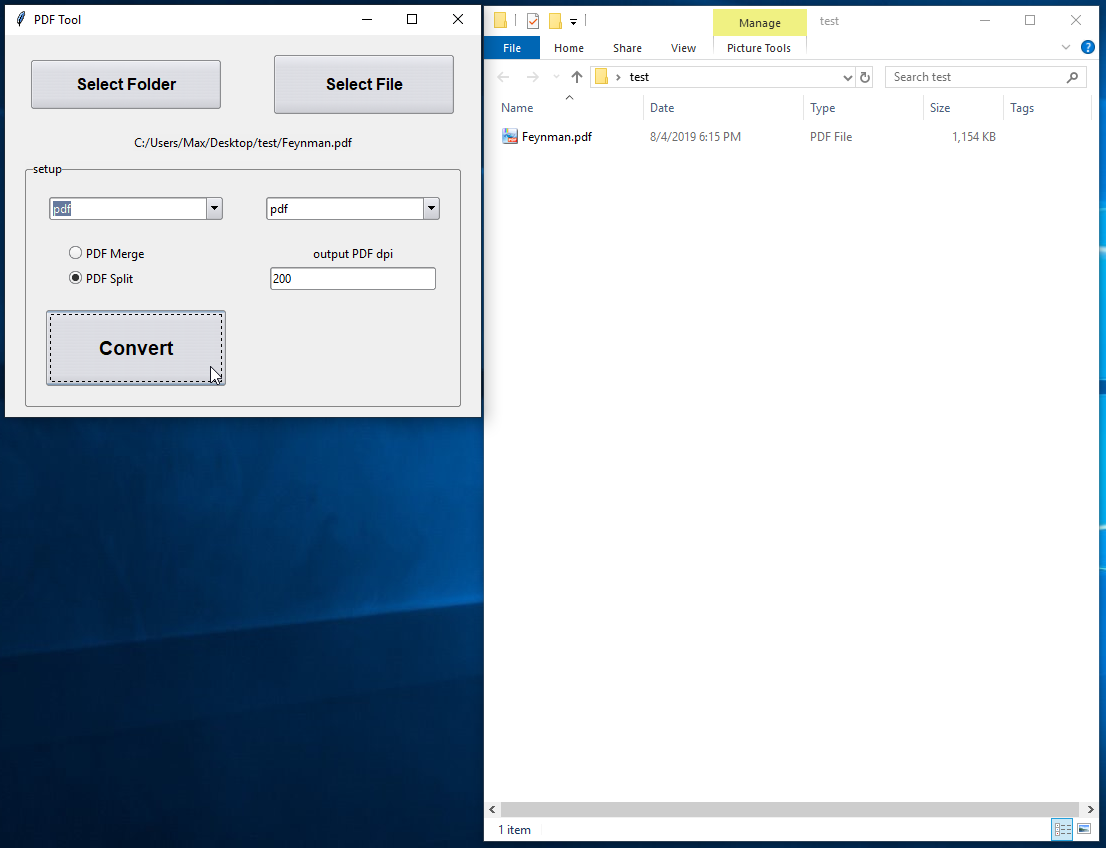
\includegraphics[width=16cm,height=6.8cm,trim={1mm 11.3cm 1.5mm 1mm},clip]{PDFSplit.png}
    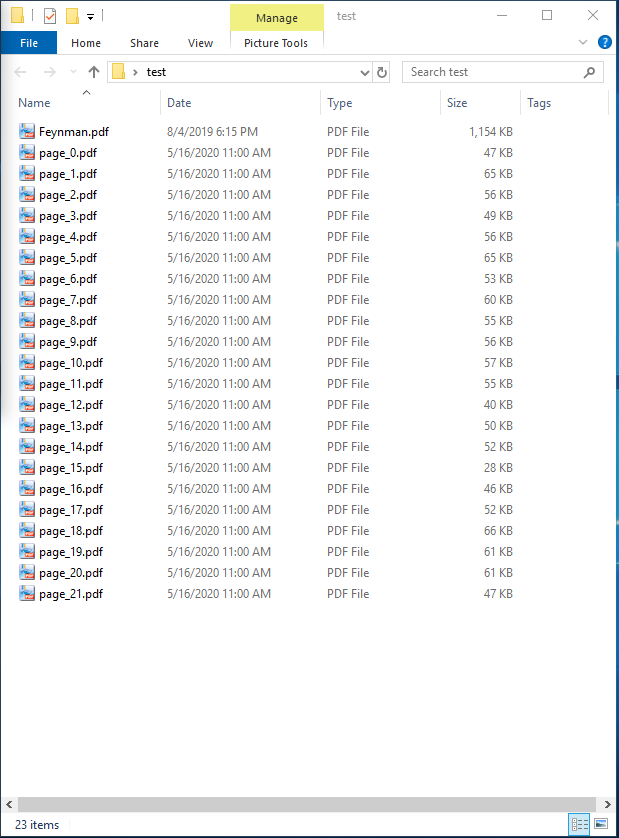
\includegraphics[width=10cm,height=8cm,trim={0 10cm 0.8mm 0},clip]{PDFSplited.png}
\end{center}

\item PDF Merge: select folder -- pdf to pdf -- PDF Merge -- convert:

\begin{center}
    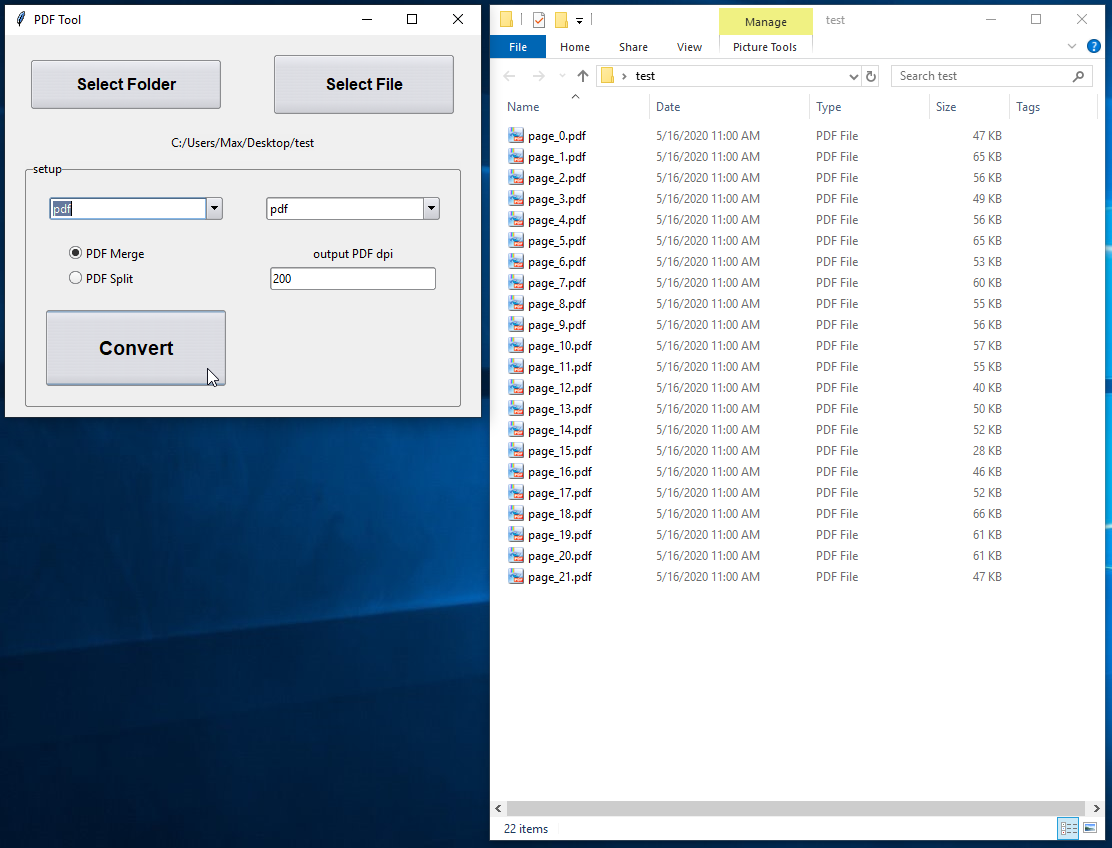
\includegraphics[width=16cm,height=6.8cm,trim={1mm 11.3cm 1.5mm 1mm},clip]{PDFMerge.png}
    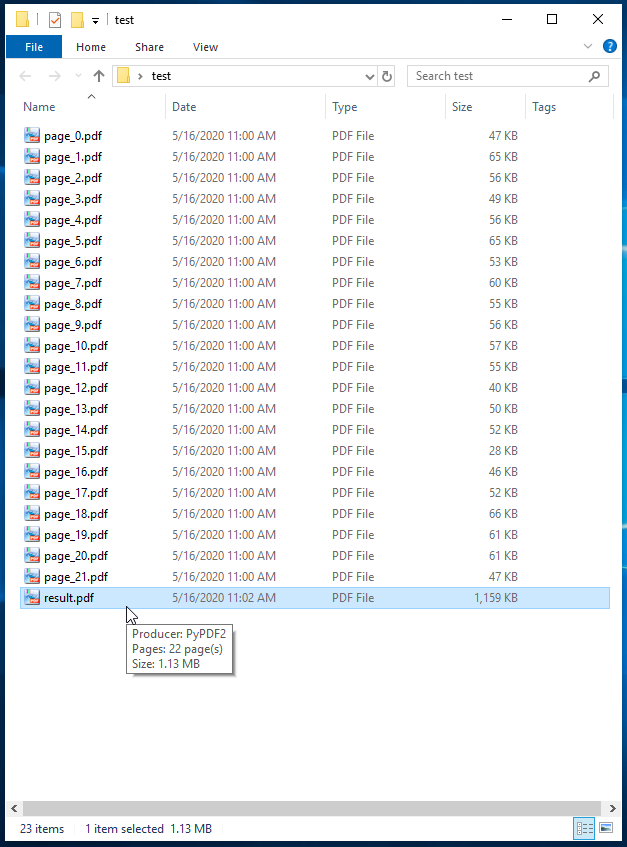
\includegraphics[width=10cm,height=7cm,trim={1mm 5cm 0.8mm 8cm},clip]{PDFMerged.png}
\end{center}

\item Image to PDF: select folder/file -- jpg/png to pdf -- convert:

\begin{center}
    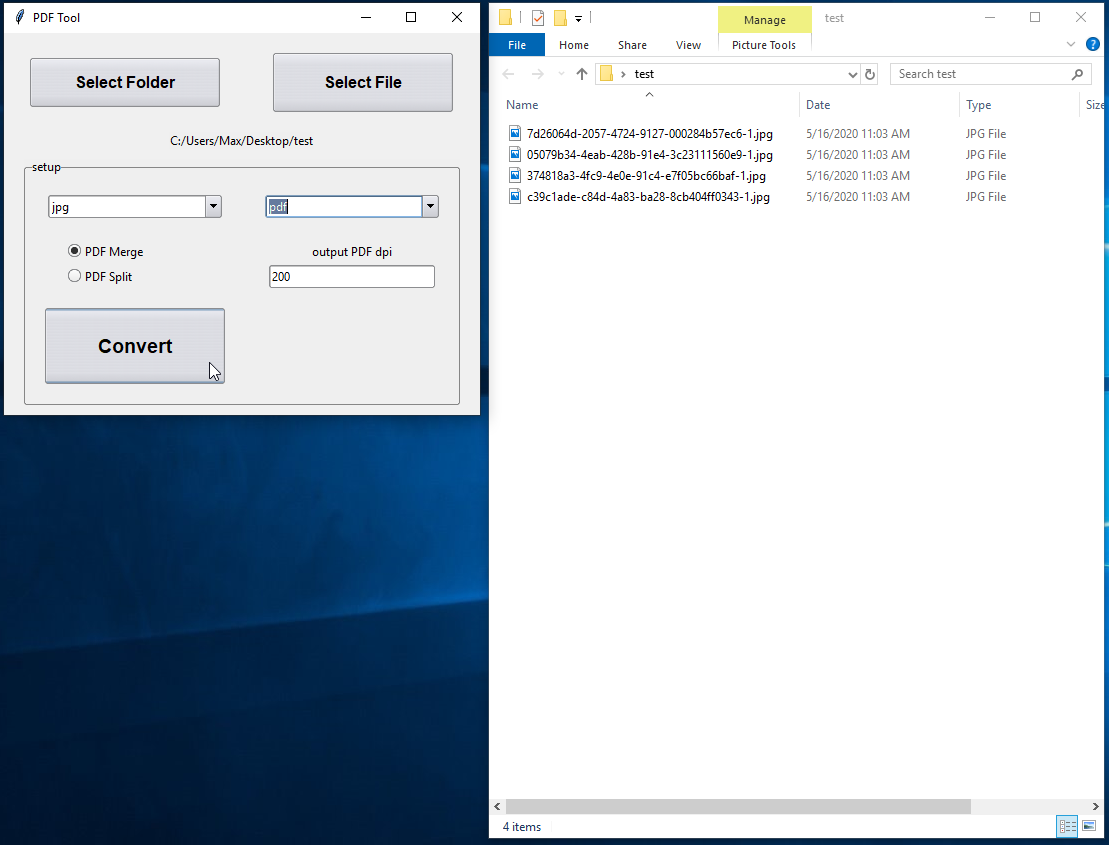
\includegraphics[width=16cm,height=6.8cm,trim={0 11.3cm 1mm 0},clip]{JpgToPDF.png}
    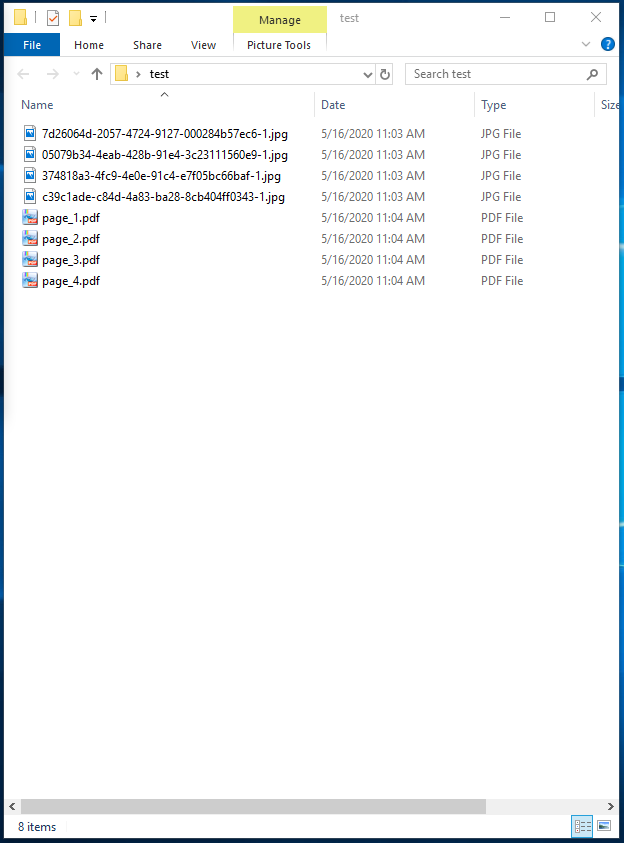
\includegraphics[width=10cm,height=5cm,trim={1mm 14.5cm 0.8mm 2.5cm},clip]{JpgToPDFFinished.png}
\end{center}

\item PDF to Image: select folder/file -- pdf to jpg/png -- convert:

\begin{center}
    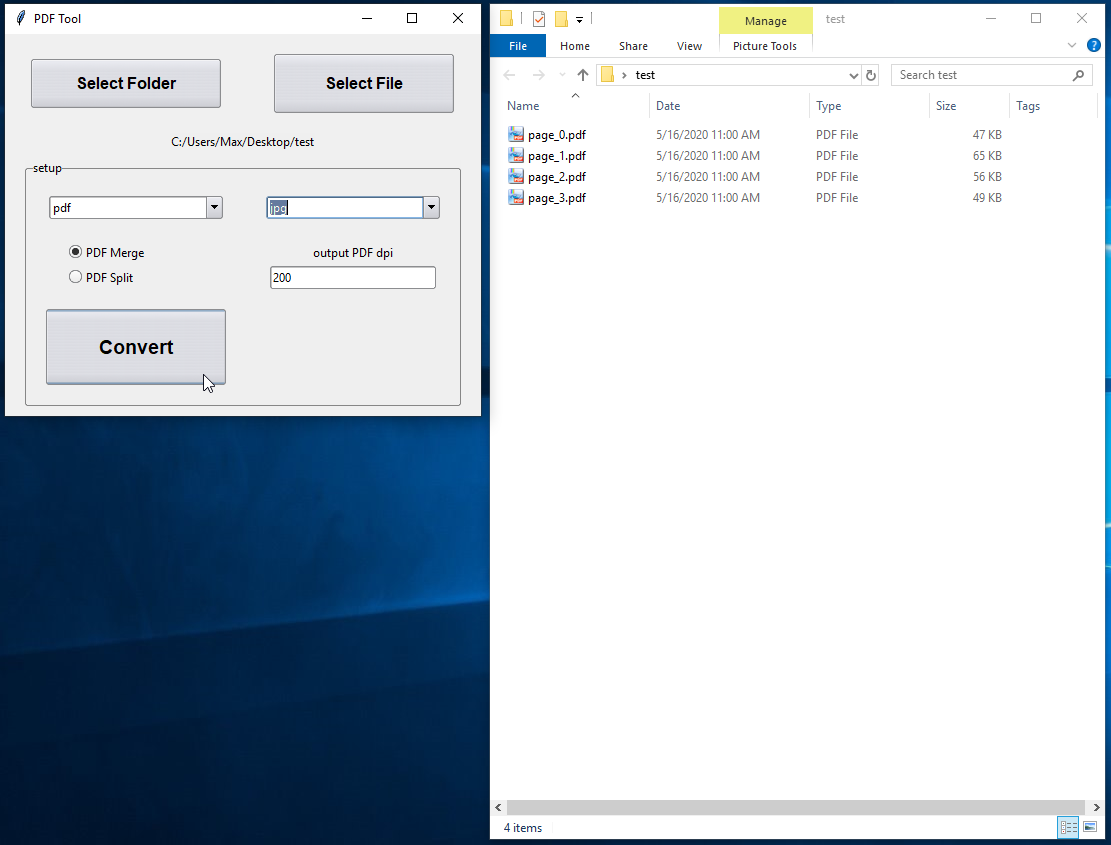
\includegraphics[width=16cm,height=6.8cm,trim={0 11.3cm 1mm 0},clip]{PDFToJpg.png}
    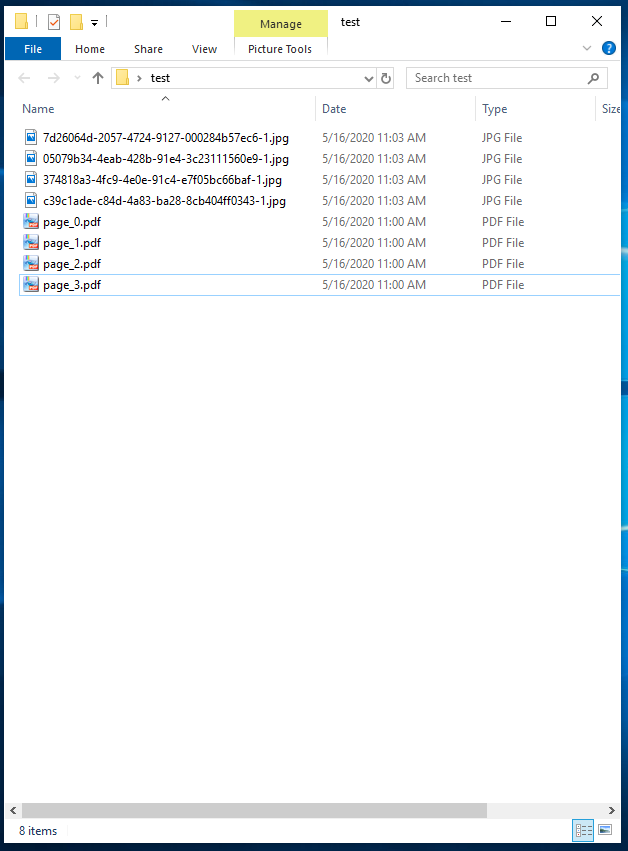
\includegraphics[width=10cm,height=5cm,trim={0 14.5cm 1.2mm 2.5cm},clip]{PDFToJpgFinished.png}
\end{center}

\end{itemize}
\vspace{12mm}
\begin{flushright}
    Max Liu \par
    \url{max.liu@outlook.com}\par
    2020.05.16   
\end{flushright}


\end{document}